
% Under the context of natural language processing, the correlation between different tokens~(words) follows the order of logic. 
% Autoregressive language models~(ARM) use causal masks to enforce causality throughout the inference process. 
% Interestingly, our observation shows that the context correlation persists even within the non-causal, fully bidirectional attention of the well-trained diffusion language models. 
% During the steps of DLMs, the contribution of masked tokens to earlier unmasked ``clean'' tokens diminishes rapidly over denoising steps. This insight enables us to exploit caching the Key and Value states of the ``clean'' tokens and reuse them across future steps without noticeable quality degradation, namely, the \texttt{FreeCache}.


% \textit{Initial clean token caching}: 
% Naturally, the input sequence $x_T$ of the diffusion model can be split into prompt tokens $x_P$ and masked dirty tokens $x_G$. 
% Correspondingly, the input query, and key states tensors of each attention block includes the pair of $[Q_P, Q_G]$, $[K_P, K_G]$, respectively. 
% \begin{align}
% Q &= \begin{bmatrix}Q_P \\[4pt] Q_G\end{bmatrix}, 
% \quad
% K = \begin{bmatrix}K_P \\[4pt] K_G\end{bmatrix}, 
% \end{align}
% Therefore, the computation of attention can be represented as the block-wise format as follow: 
% \begin{align}\label{eq:block_diff}
% Q\,K^T
% &= \begin{bmatrix}
% Q_P\,K_P^T & Q_P\,K_G^T \\[6pt]
% Q_G\,K_P^T & Q_G\,K_G^T
% \end{bmatrix},
% \end{align}

% We characterize the impact of each block of $Q\,K^T$ throughout the entire diffusion process~(step 1 to $T$) based on the SoTA Dream-7B-Instruct~\cite{dream2025} model. 
% As shown in Figure~\ref{fig:freecache_rationale},$[Q_P\,K_P^T]_t$ is highly correlated~(within 0.9 and 1.0) with the initial state at each step of the diffusion process, in comparison to other partial attention blocks. 
% Such observation motivates us to exploit the plausibility of caching the Key States that correspond to the prompt tokens of input. In other words, the cached $K_P$ approximates the $Q_P\,K_P^T$. 

% We adopt a \textbf{block-wise} generation scheme. We pre-allocate a K/V cache for the full context length (prompt + generation) and populate it in one initial forward pass. The prompt's K/V is then frozen. Generation proceeds block-by-block. The current block's Query attends to the entire, full-context K/V cache. This cache is dynamically updated by recomputing the current block's K/V, which is then frozen once fully unmasked. For each active block, we run denoising while letting its Queries attend to the full K/V cache (frozen prompt + previously finalized blocks + a cached initialization for future masked tokens). Once the block becomes fully unmasked and stable, we compute its K/V once, freeze them into the global cache, and advance to the next block. This avoids recomputing attention over the entire sequence of length $L$ at every step: only the Queries for the current block of size $B$ are recomputed, while K/V elsewhere are reused. Consequently, per-step compute scales with $B$ rather than $L$. According to Eq~\ref{eq:block_diff}, this reuse preserves the $Q_P\,K_P^T$ interaction and approximates $Q_P\,K_G^T$, yielding substantial speedups with minimal quality impact. 

\subsubsection{FreeCache: Reducing Window Caching for DLM Inference}
\label{sec:freecache}
A key insight for optimizing the generation process in Diffusion Language Models is that the Key and Value (KV) projections for the clean portions of a sequence exhibit high temporal stability. Although these projections are not strictly unchanging, they quickly converge and undergo only negligible changes once a token is finalized.

Figure 2 shows a heatmap that validates the rationale behind our FreeCache method: the temporal stability of KV projections for clean tokens. The y-axis represents the denoising step and the x-axis represents the token position, while the color intensity shows the similarity of a token's value projection to its previous step. Bright yellow indicates high similarity (minimal change), while dark blue signifies a large difference. We observed that the prompt region remains stable across denoising steps, and the generation region illustrates how tokens transition from a low-similarity, unstable state (dark blue) to a high-similarity, stable state (bright yellow) as they become unmasked.

% \begin{figure}[t!]
\begin{figure}[H]
    \centering
    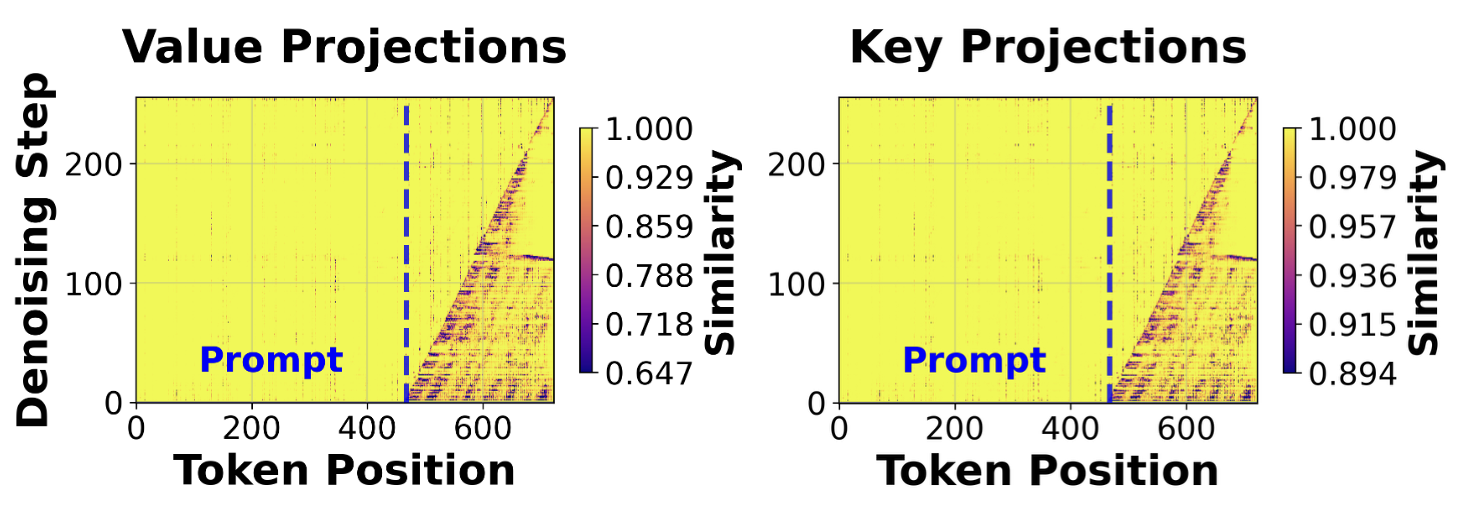
\includegraphics[width=1\linewidth]{sections/method/figures/kv_projections.png}
    \caption{Rationale behind the proposed FreeCache: The variation of K and V projections of clean tokens is small throughout the subsequent diffusion steps. }
    \label{fig:freecache_rationale}
\end{figure}




To exploit this, we propose \texttt{FreeCache}, a reducing window caching strategy where the set of actively computed tokens dynamically shrinks as blocks of the sequence are finalized. The algorithm proceeds as follows: \textbf{Initialization and Partitioning:} The post-prompt generation sequence is partitioned into fixed-size blocks ($B_1, ..., B_N$), and an initial forward pass computes and saves the full KV projections for the entire sequence (prompt + all blocks). \textbf{Windowed Re-computation:} To generate a block $B_i$, the \textbf{active computation window} is defined as $B_i$ and all subsequent blocks ($B_{i+1}, ..., B_N$). KV projections are recomputed only for tokens within this window until $B_i$ is fully unmasked, using all prior frozen blocks and the prompt as context. \textbf{Progressive Caching:} Upon completion of a block $B_i$, its KV projections are \textbf{frozen} for subsequent steps. The active window then shrinks to exclude this block for all subsequent generation steps.

This cascaded approach means that the computational cost per step progressively decreases throughout the inference process, as the active window shrinks with each completed block. This effectively reduces the overall computational overhead, especially for long sequences.


We quantify the performance degradation caused by the \texttt{FreeCache} in Figure~\ref{fig:kvcache} with the 8-shot GSM8K dataset. 
The reducing window caching strategy introduces up to 5$\times$ speedup compared to the vanilla Dream-7B, while preserving the minimal accuracy drop. As shown in Table~\ref{tab:freecache_results}, the proposed FreeCache achieves up to 4.42$\times$ speedup for Dream-7B-Instruct and 6.32$\times$ for LLaDA-8B-Instruct, while maintaining accuracy close to the baseline. We solidify the performance of the proposed method in Section~\ref{sec:res} with further analysis with benchmarks across different domains.





% Although the speedup is achieved with the proposed caching strategy, we further propose a novel method to completely recover the accuracy degradation while exploit the acceleration even further. 
% \textit{Blockwise semi-autoregressive diffusion}: 
% For the remaining masked positions we split them into contiguous blocks of size 
% B. At each step, we only pass the current block to the model. We iteratively repeat the denoising process on the current block until the current block is fully unmasked, and then cache the projected KV corresponding to this block and move on to the next block. This keeps generation within local block diffusive, \zhanqiu{correct word?}, while introducing blockwise auto-regressiveness. This semi-autoregressive diffusion approach reduce input length in subsequent steps from $L$ to $B$, where $B$ is a user-defined value smaller or equal to the context length. 

% \textit{Early exit:} On top of block-wise caching, we implemented an early stopping mechanism that exits generation when an end-of-text token is unmasked and all tokens before the eos are unmasked. 


% In practice, FreeCache \zhanqiu{Rename} yields 5× \zhanqiu{Fill with more data} reduction in generation latency compared with the baseline Dream 7B without measurable degradation in accuracy. It significantly reduces the computation for long sequence generation. Detailed results are presented in Section~\ref{sec: experiments}.

% The semi-autoregressive generation and early stopping enhances each other: we observe that with fully diffusion language model, when the provision context length is longer than the actual generated token, it tends to unmask later tokens as EOS tokens before unmasking actually meaningful tokens (this is especially obvious in tasks like Hellaswag)

% Algorithm:
% 1. In the first denoising step, we pass in the full sequence. We cache the projected keys and values of the cleaning tokens (i.e., the prompt tokens in generation tasks)

% 2. For later steps, splitting the target masked sequence into several blocks and generating them from left right. Caching the each block when they become fully unmasked. This keeps generation within local ... diffusive while introducing blockwise auto-regressiveness. This semi-autoregressive diffusion approach reduce input length in subsequent steps from $L$ to $B$, where $B$ is a user-defined value smaller or equal to the context length. 

% 3. In addition to caching, we also implemented an early stopping mechanism that exits generation when an eos token is unmasked and all tokens before the eos are unmasked. The semi-autoregressive generation and early stopping enhances each other: we observe that with fully diffusion language model, when the provision context length is longer than the actual generated token, it tends to unmask later tokens as EOS tokens before unmasking actually meaningful tokens (this is especially obvious in tasks like Hellaswag)



% \begin{figure}[h!]
%   \centering
%   \includegraphics[width=0.95\columnwidth]{sections/method/kvcache_system.png}
%   \vspace{-0.5em}
%   \caption{
%     \textbf{Memory–compute tradeoffs across generation paradigms.} 
%     Left: AR decoding is memory-bound due to the growing KV cache. 
%     Middle: DLM decoding is compute-bound due to repeated full-sequence forward passes. 
%     Right: Our method with KV caching selectively reuses KV projections for clean tokens, striking a balance between reuse and recomputation.
%   }
%   \label{fig:kvcache-compare}
% \end{figure}
